\documentclass[12pt,a4paper]{article}

% Packages
\usepackage[margin=1in]{geometry}
\usepackage{graphicx}
\usepackage{amsmath}
\usepackage{amssymb}
\usepackage{float}
\usepackage{subcaption}
\usepackage{booktabs}
\usepackage{siunitx}
\usepackage{listings}
\usepackage{xcolor}
\usepackage{hyperref}
\usepackage{fancyhdr}
\usepackage{titlesec}
\usepackage{multirow}

% Code listing setup
\lstset{
    basicstyle=\ttfamily\footnotesize,
    keywordstyle=\color{blue},
    commentstyle=\color{green!60!black},
    stringstyle=\color{red},
    numbers=left,
    numberstyle=\tiny\color{gray},
    frame=single,
    breaklines=true,
    captionpos=b,
    showstringspaces=false
}

% Header and footer
\pagestyle{fancy}
\fancyhf{}
\rhead{Active Suspension System}
\lhead{Systems Simulation Laboratory}
\rfoot{Page \thepage}

% Title formatting
\titleformat{\section}{\Large\bfseries}{\thesection}{1em}{}
\titleformat{\subsection}{\large\bfseries}{\thesubsection}{1em}{}

\begin{document}

% Title Page
\begin{titlepage}
    \centering
    \vspace*{1cm}
    
    % \includegraphics[width=0.3\textwidth]{logo.png}\\[1cm]
    
    {\LARGE\bfseries ELECTRICAL \& ELECTRONICS ENGINEERING\\[0.3cm]}
    {\Large Manipal Institute of Technology\\[0.5cm]}
    {\large Manipal - 576104\\[1cm]}
    
    \rule{\linewidth}{0.5mm}\\[0.4cm]
    {\huge\bfseries ACTIVE SUSPENSION SYSTEM\\[0.2cm]
    Design and Performance Analysis\\[0.4cm]}
    \rule{\linewidth}{0.5mm}\\[1.5cm]
    
    {\Large\textbf{Systems Simulation Laboratory}\\[0.2cm]
    ELE 3142\\[0.5cm]}
    
    {\large 5th Semester B.Tech. (E \& E Engineering)\\[1.5cm]}
    
    % Team Members Table
    \begin{table}[H]
    \centering
    \begin{tabular}{|c|l|c|c|}
    \hline
    \textbf{S.No} & \textbf{Name} & \textbf{Registration No.} & \textbf{Roll No.} \\ \hline
    1 & Gonugondla Veera Manikanta & 230906450 & 54 \\ \hline
    2 & Rounak Pradhan & 230906492 & 60 \\ \hline
    \end{tabular}
    \end{table}
    
    \vfill
    
    {\large July -- December 2025}
    
\end{titlepage}

% Individual Contributions
\newpage
\section*{Individual Contributions}
\addcontentsline{toc}{section}{Individual Contributions}

\begin{table}[H]
\centering
\begin{tabular}{|l|p{10cm}|}
\hline
\textbf{Team Member} & \textbf{Contribution} \\ \hline
\multirow{3}{*}{\textbf{Gonugondla Veera Manikanta}} 
& \vspace{2pt}• MATLAB/Simulink model development and implementation \\ 
& • System parameter definition and configuration \\
& • Simulink block diagram design and subsystem creation \\
& • Simulation execution and data collection \\
& • MATLAB script development for Bode plot analysis \\ \hline
\multirow{3}{*}{\textbf{Rounak Pradhan}} 
& \vspace{2pt}• Technical report writing and documentation \\ 
& • Results analysis and interpretation \\
& • Performance metrics calculation and comparison \\
& • Literature review and theoretical background \\
& • LaTeX document preparation and formatting \\ \hline
\end{tabular}
\caption{Distribution of work among team members}
\end{table}

\textbf{Note:} Both team members collaborated on the project conceptualization, design decisions, and final review of deliverables.

% Abstract
\newpage
\section*{Abstract}
\addcontentsline{toc}{section}{Abstract}

This report presents the design, analysis, and simulation of an active suspension system for automotive applications. The study compares the performance of passive and active suspension configurations using a quarter-car model. A Proportional-Integral-Derivative (PID) controller is designed to actively control the suspension forces, aiming to improve ride comfort and handling characteristics. Mathematical modeling using transfer functions and state-space representations is developed, followed by comprehensive frequency and time domain analysis. Simulation results demonstrate that the active suspension system achieves significant improvements in vibration isolation, with a peak magnitude reduction of \SI{15.24}{dB} compared to the passive system. The findings validate the effectiveness of active control strategies in enhancing vehicle suspension performance.

\textbf{Keywords:} Active suspension, PID control, Quarter-car model, MATLAB/Simulink, Frequency response analysis

% Table of Contents
\newpage
\tableofcontents

% List of Figures
\newpage
\listoffigures

% List of Tables
\listoftables

% Main Content
\newpage
\section{Introduction}

\subsection{Background}
Vehicle suspension systems play a critical role in ensuring passenger comfort, vehicle stability, and road handling. Traditional passive suspension systems use fixed spring and damper characteristics that represent a compromise between ride comfort and handling performance. Active suspension systems overcome these limitations by incorporating actuators and control systems that can adapt to varying road conditions and driving scenarios in real-time.

\subsection{Motivation}
The development of active suspension systems addresses several key challenges:
\begin{itemize}
    \item Reduction of body oscillations during acceleration, braking, and cornering
    \item Improved isolation from road irregularities and vibrations
    \item Enhanced vehicle stability and safety
    \item Adaptability to different loading conditions and road profiles
\end{itemize}

\subsection{Objectives}
The primary objectives of this project are:
\begin{enumerate}
    \item To develop a mathematical model of a quarter-car suspension system
    \item To design a PID controller for active suspension control
    \item To implement the system in MATLAB/Simulink environment
    \item To analyze and compare the performance of passive and active configurations
    \item To evaluate system response through frequency and time domain analysis
\end{enumerate}

\subsection{Scope}
This study focuses on a simplified quarter-car model representing one corner of the vehicle. The analysis includes:
\begin{itemize}
    \item Transfer function and state-space modeling
    \item PID controller design using velocity feedback
    \item Bode plot analysis for frequency response characterization
    \item Time-domain simulations for various road inputs
    \item Performance metrics evaluation (body acceleration, suspension travel, settling time)
\end{itemize}

\section{System Modeling}

\subsection{Quarter-Car Model}
The quarter-car model represents the vertical dynamics of one corner of a vehicle. The system consists of two masses connected by spring-damper elements, as illustrated in Figure \ref{fig:simulink_model}.

\textbf{Model components:}
\begin{itemize}
    \item \textbf{Sprung mass ($m_s$):} Vehicle body mass (\SI{300}{kg})
    \item \textbf{Unsprung mass ($m_{us}$):} Wheel assembly mass (\SI{40}{kg})
    \item \textbf{Suspension spring ($k_s$):} Spring connecting body and wheel (\SI{18000}{N/m})
    \item \textbf{Suspension damper ($c_s$):} Damping element in suspension (\SI{1200}{N.s/m})
    \item \textbf{Tire spring ($k_t$):} Tire stiffness (\SI{195000}{N/m})
    \item \textbf{Tire damper ($c_t$):} Tire damping (\SI{75}{N.s/m})
    \item \textbf{Control force ($F_c$):} Active actuator force (variable)
\end{itemize}

\subsection{Mathematical Equations}

Applying Newton's second law to both masses yields the following equations of motion:

\textbf{Sprung mass (vehicle body):}
\begin{equation}
    m_s \ddot{x}_s = -k_s(x_s - x_{us}) - c_s(\dot{x}_s - \dot{x}_{us}) + F_c
    \label{eq:sprung_mass}
\end{equation}

\textbf{Unsprung mass (wheel assembly):}
\begin{equation}
    m_{us} \ddot{x}_{us} = k_s(x_s - x_{us}) + c_s(\dot{x}_s - \dot{x}_{us}) - k_t(x_{us} - x_r) - c_t(\dot{x}_{us} - \dot{x}_r) - F_c
    \label{eq:unsprung_mass}
\end{equation}

where:
\begin{align*}
    x_s &= \text{Sprung mass displacement (m)} \\
    x_{us} &= \text{Unsprung mass displacement (m)} \\
    x_r &= \text{Road profile input (m)} \\
    F_c &= \text{Active control force (N)}
\end{align*}

\subsection{Transfer Function Representation}

Taking the Laplace transform of equations (\ref{eq:sprung_mass}) and (\ref{eq:unsprung_mass}) and manipulating, we obtain the transfer function from road input to body displacement for the passive system:

\begin{equation}
    G_p(s) = \frac{X_s(s)}{X_r(s)} = \frac{(c_s s + k_s)(c_t s + k_t)}{D(s)}
    \label{eq:passive_tf}
\end{equation}

where the denominator polynomial is:
\begin{align}
    D(s) = &\, m_s m_{us} s^4 + (m_s c_t + m_{us} c_s) s^3 \nonumber \\
    &+ (m_s k_t + m_{us} k_s + c_s c_t) s^2 \nonumber \\
    &+ (c_s k_t + c_t k_s) s + k_s k_t
\end{align}

\subsection{System Parameters}

The physical parameters used in this study are presented in Table \ref{tab:parameters}.

\begin{table}[H]
\centering
\caption{Quarter-car suspension system parameters}
\label{tab:parameters}
\begin{tabular}{@{}lll@{}}
\toprule
\textbf{Parameter} & \textbf{Value} & \textbf{Unit} \\ \midrule
Sprung mass, $m_s$ & 300 & kg \\
Unsprung mass, $m_{us}$ & 40 & kg \\
Suspension spring stiffness, $k_s$ & 18,000 & N/m \\
Suspension damping coefficient, $c_s$ & 1,200 & N·s/m \\
Tire stiffness, $k_t$ & 195,000 & N/m \\
Tire damping coefficient, $c_t$ & 75 & N·s/m \\ \bottomrule
\end{tabular}
\end{table}

These parameters are representative of a typical passenger vehicle and were selected based on standard automotive engineering practices.

\section{Controller Design}

\subsection{Control Strategy}
The active suspension system employs a PID controller with velocity feedback to generate the control force. The control law is given by:

\begin{equation}
    F_c(s) = C_{PID}(s) \cdot \left( V_{desired}(s) - V_{actual}(s) \right)
    \label{eq:control_law}
\end{equation}

where $V_{actual}(s) = s \cdot X_s(s)$ is the body velocity. For vibration suppression, the desired velocity is set to zero.

\subsection{PID Controller Structure}

The PID controller transfer function with derivative filter is:

\begin{equation}
    C_{PID}(s) = K_p + \frac{K_i}{s} + \frac{K_d N s}{s + N}
    \label{eq:pid}
\end{equation}

where:
\begin{itemize}
    \item $K_p$ = Proportional gain
    \item $K_i$ = Integral gain
    \item $K_d$ = Derivative gain
    \item $N$ = Filter coefficient (typically 100)
\end{itemize}

The derivative filter is included to prevent noise amplification at high frequencies.

\subsection{Gain Selection}

Controller gains were selected based on the following design criteria:

\begin{enumerate}
    \item \textbf{Proportional Gain ($K_p$):} Provides immediate response to velocity errors. A higher value improves transient response but may cause overshoot.
    
    \item \textbf{Integral Gain ($K_i$):} Eliminates steady-state error and improves low-frequency disturbance rejection.
    
    \item \textbf{Derivative Gain ($K_d$):} Anticipates future errors based on rate of change, improving stability and reducing overshoot.
\end{enumerate}

The selected controller gains are presented in Table \ref{tab:gains}.

\begin{table}[H]
\centering
\caption{PID controller gains}
\label{tab:gains}
\begin{tabular}{@{}ll@{}}
\toprule
\textbf{Parameter} & \textbf{Value} \\ \midrule
Proportional gain, $K_p$ & 5,000 \\
Integral gain, $K_i$ & 100 \\
Derivative gain, $K_d$ & 2,000 \\
Filter coefficient, $N$ & 100 \\ \bottomrule
\end{tabular}
\end{table}

These gains were tuned iteratively to achieve optimal performance while maintaining system stability and actuator force within practical limits.

\subsection{Closed-Loop System}

The closed-loop transfer function of the active suspension system is:

\begin{equation}
    G_a(s) = \frac{G_p(s)}{1 + C_{PID}(s) \cdot s \cdot G_p(s)}
    \label{eq:active_tf}
\end{equation}

This feedback configuration allows the controller to actively counteract disturbances and reduce body oscillations.

\section{Simulation and Analysis}

\subsection{Implementation in MATLAB/Simulink}

The system was implemented in MATLAB/Simulink following a modular approach as shown in Figure \ref{fig:simulink_model}. The complete block diagram illustrates the interconnection of all system components.

\begin{figure}[H]
    \centering
    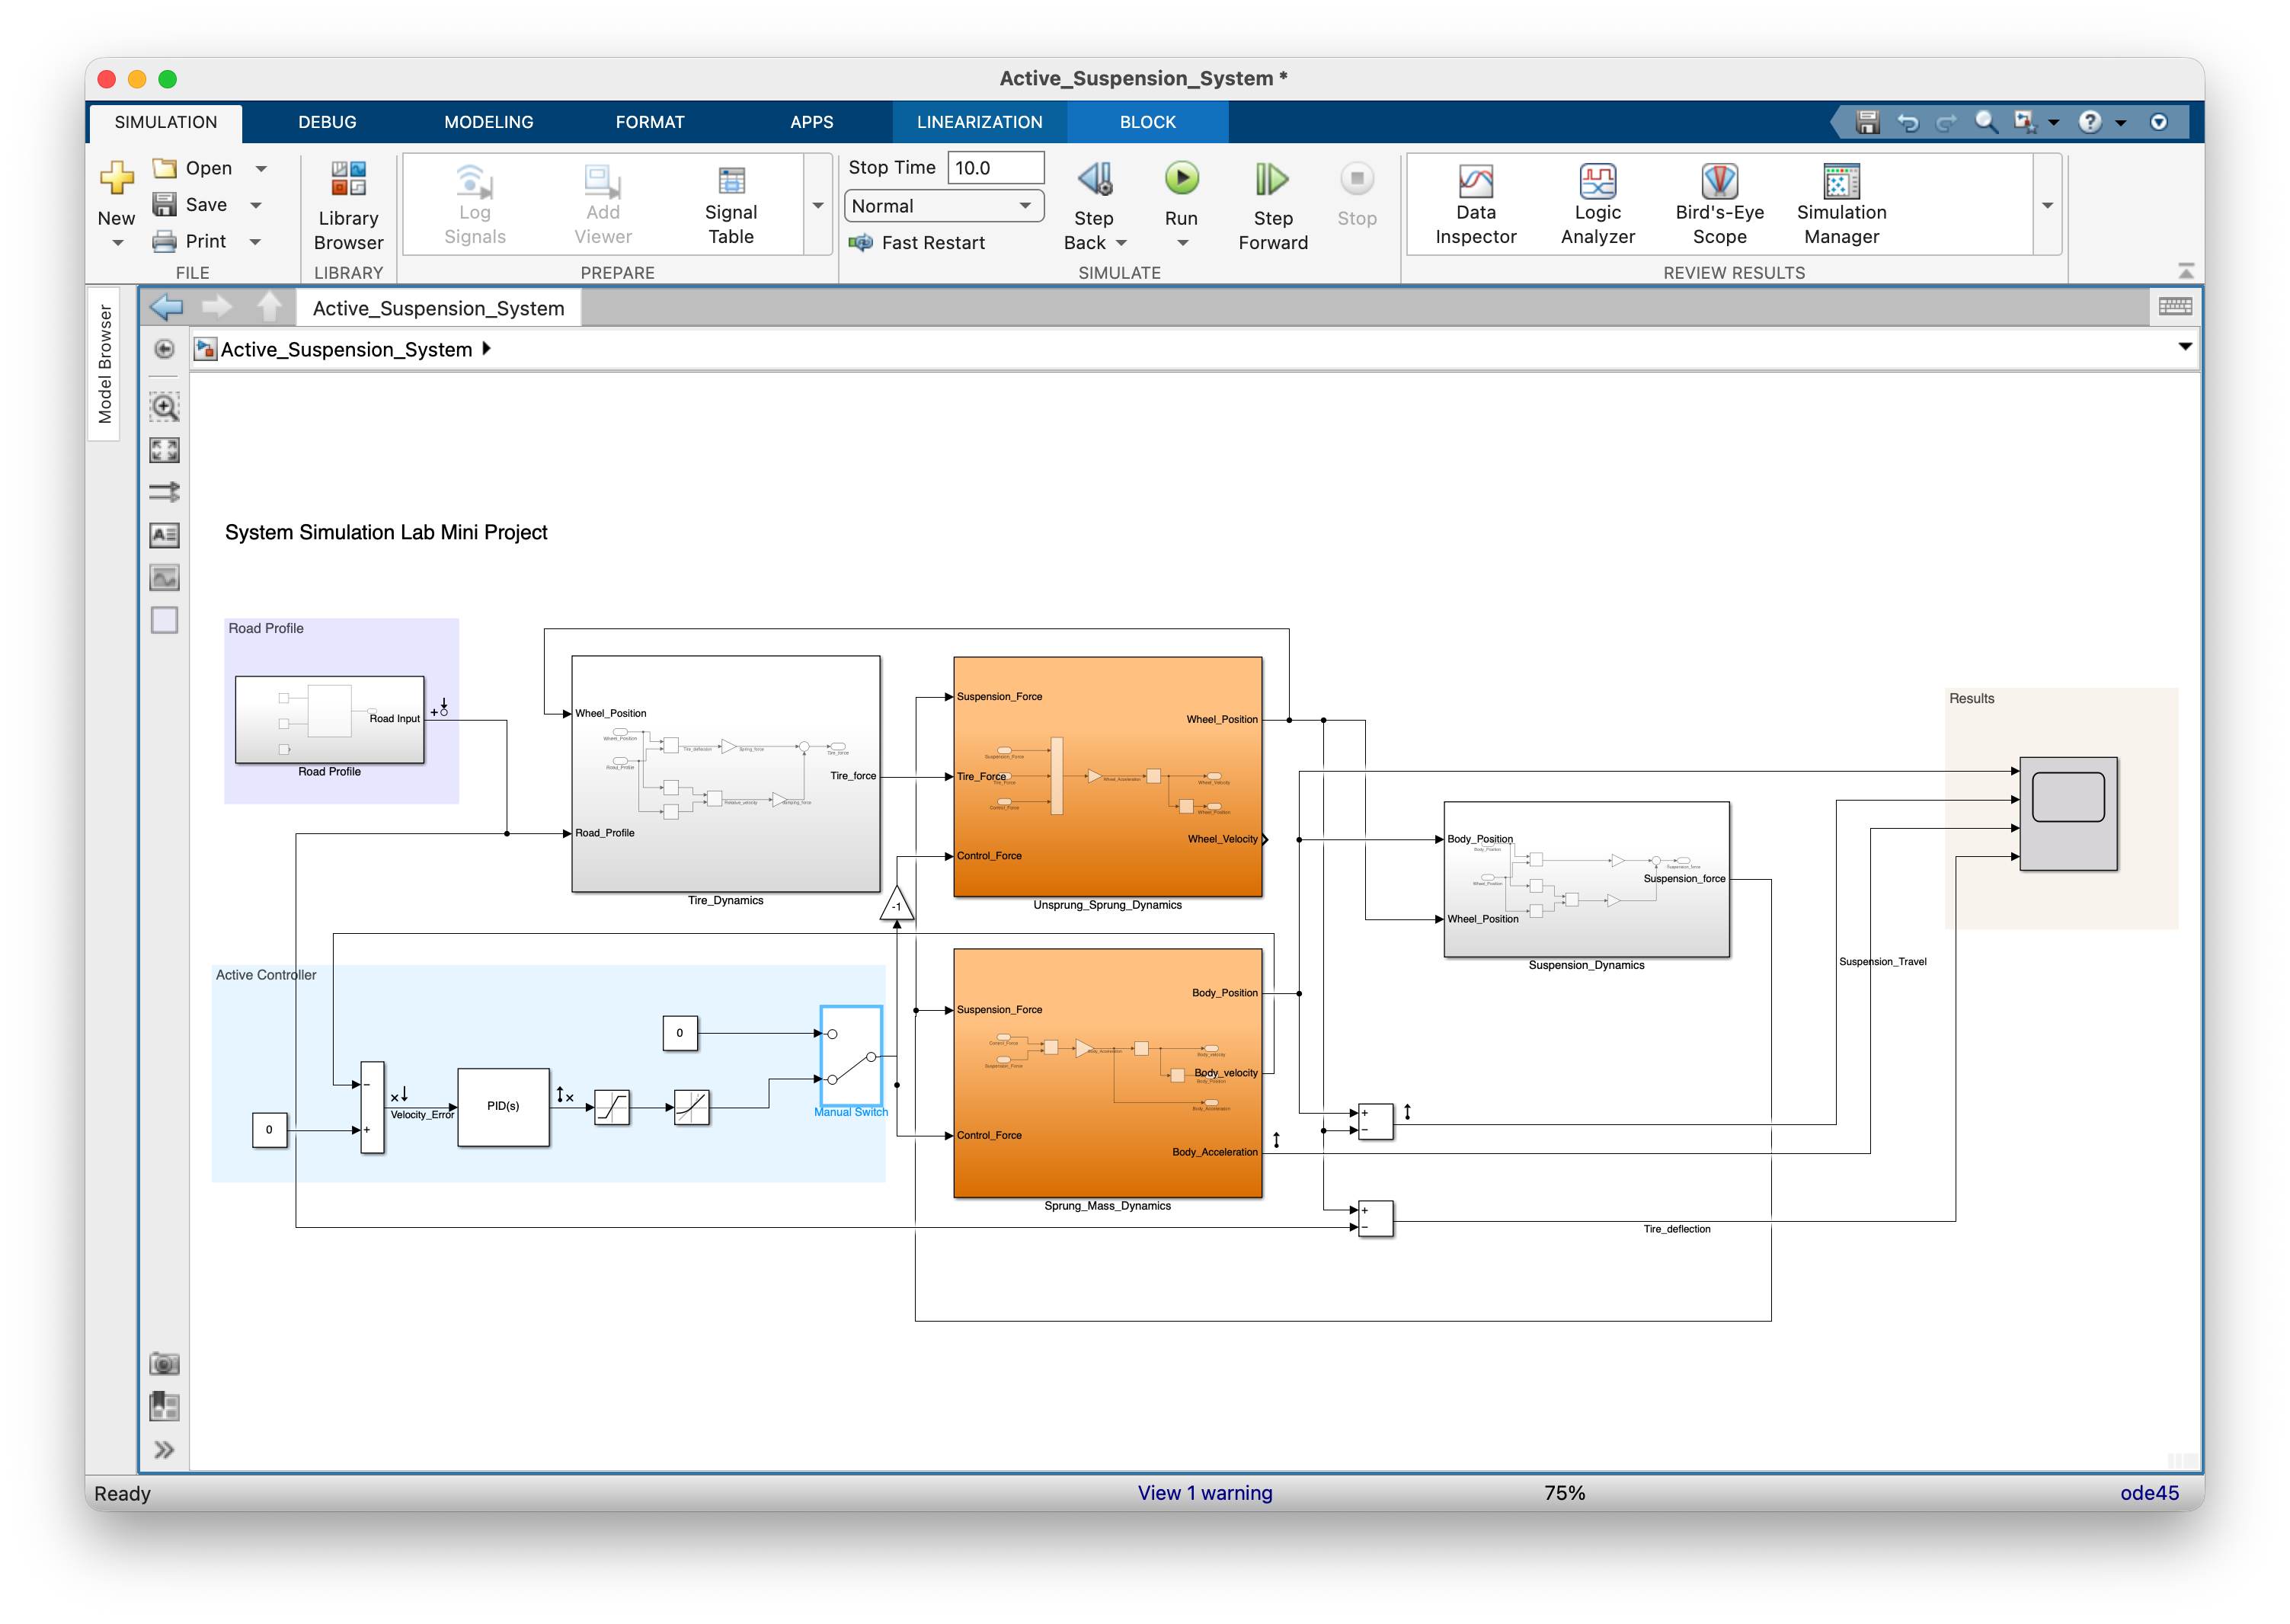
\includegraphics[width=\textwidth]{simulink_screenshot.png}
    \caption{Complete Simulink model of active suspension system showing all subsystems: Road Input, Tire Dynamics, Unsprung Mass Dynamics, Sprung Mass Dynamics, Suspension Dynamics, PID Controller, and actuator limits}
    \label{fig:simulink_model}
\end{figure}

\textbf{Key subsystems:}
\begin{enumerate}
    \item \textbf{Road Input Module:} Generates various road profiles (step bump, sinusoidal, random noise)
    \item \textbf{Tire Dynamics:} Models tire spring and damping forces between tire and road
    \item \textbf{Suspension Dynamics:} Calculates suspension spring and damping forces
    \item \textbf{Unsprung Mass Dynamics:} Computes wheel assembly motion
    \item \textbf{Sprung Mass Dynamics:} Computes vehicle body motion
    \item \textbf{PID Controller:} Generates active control force based on velocity error
    \item \textbf{Actuator Limits:} Implements saturation (±5000 N) and rate limiting
\end{enumerate}

\subsection{Time Domain Response}

The time-domain responses of both passive and active systems are compared for a step road input in Figures \ref{fig:passive_response} and \ref{fig:active_response}.

\begin{figure}[H]
    \centering
    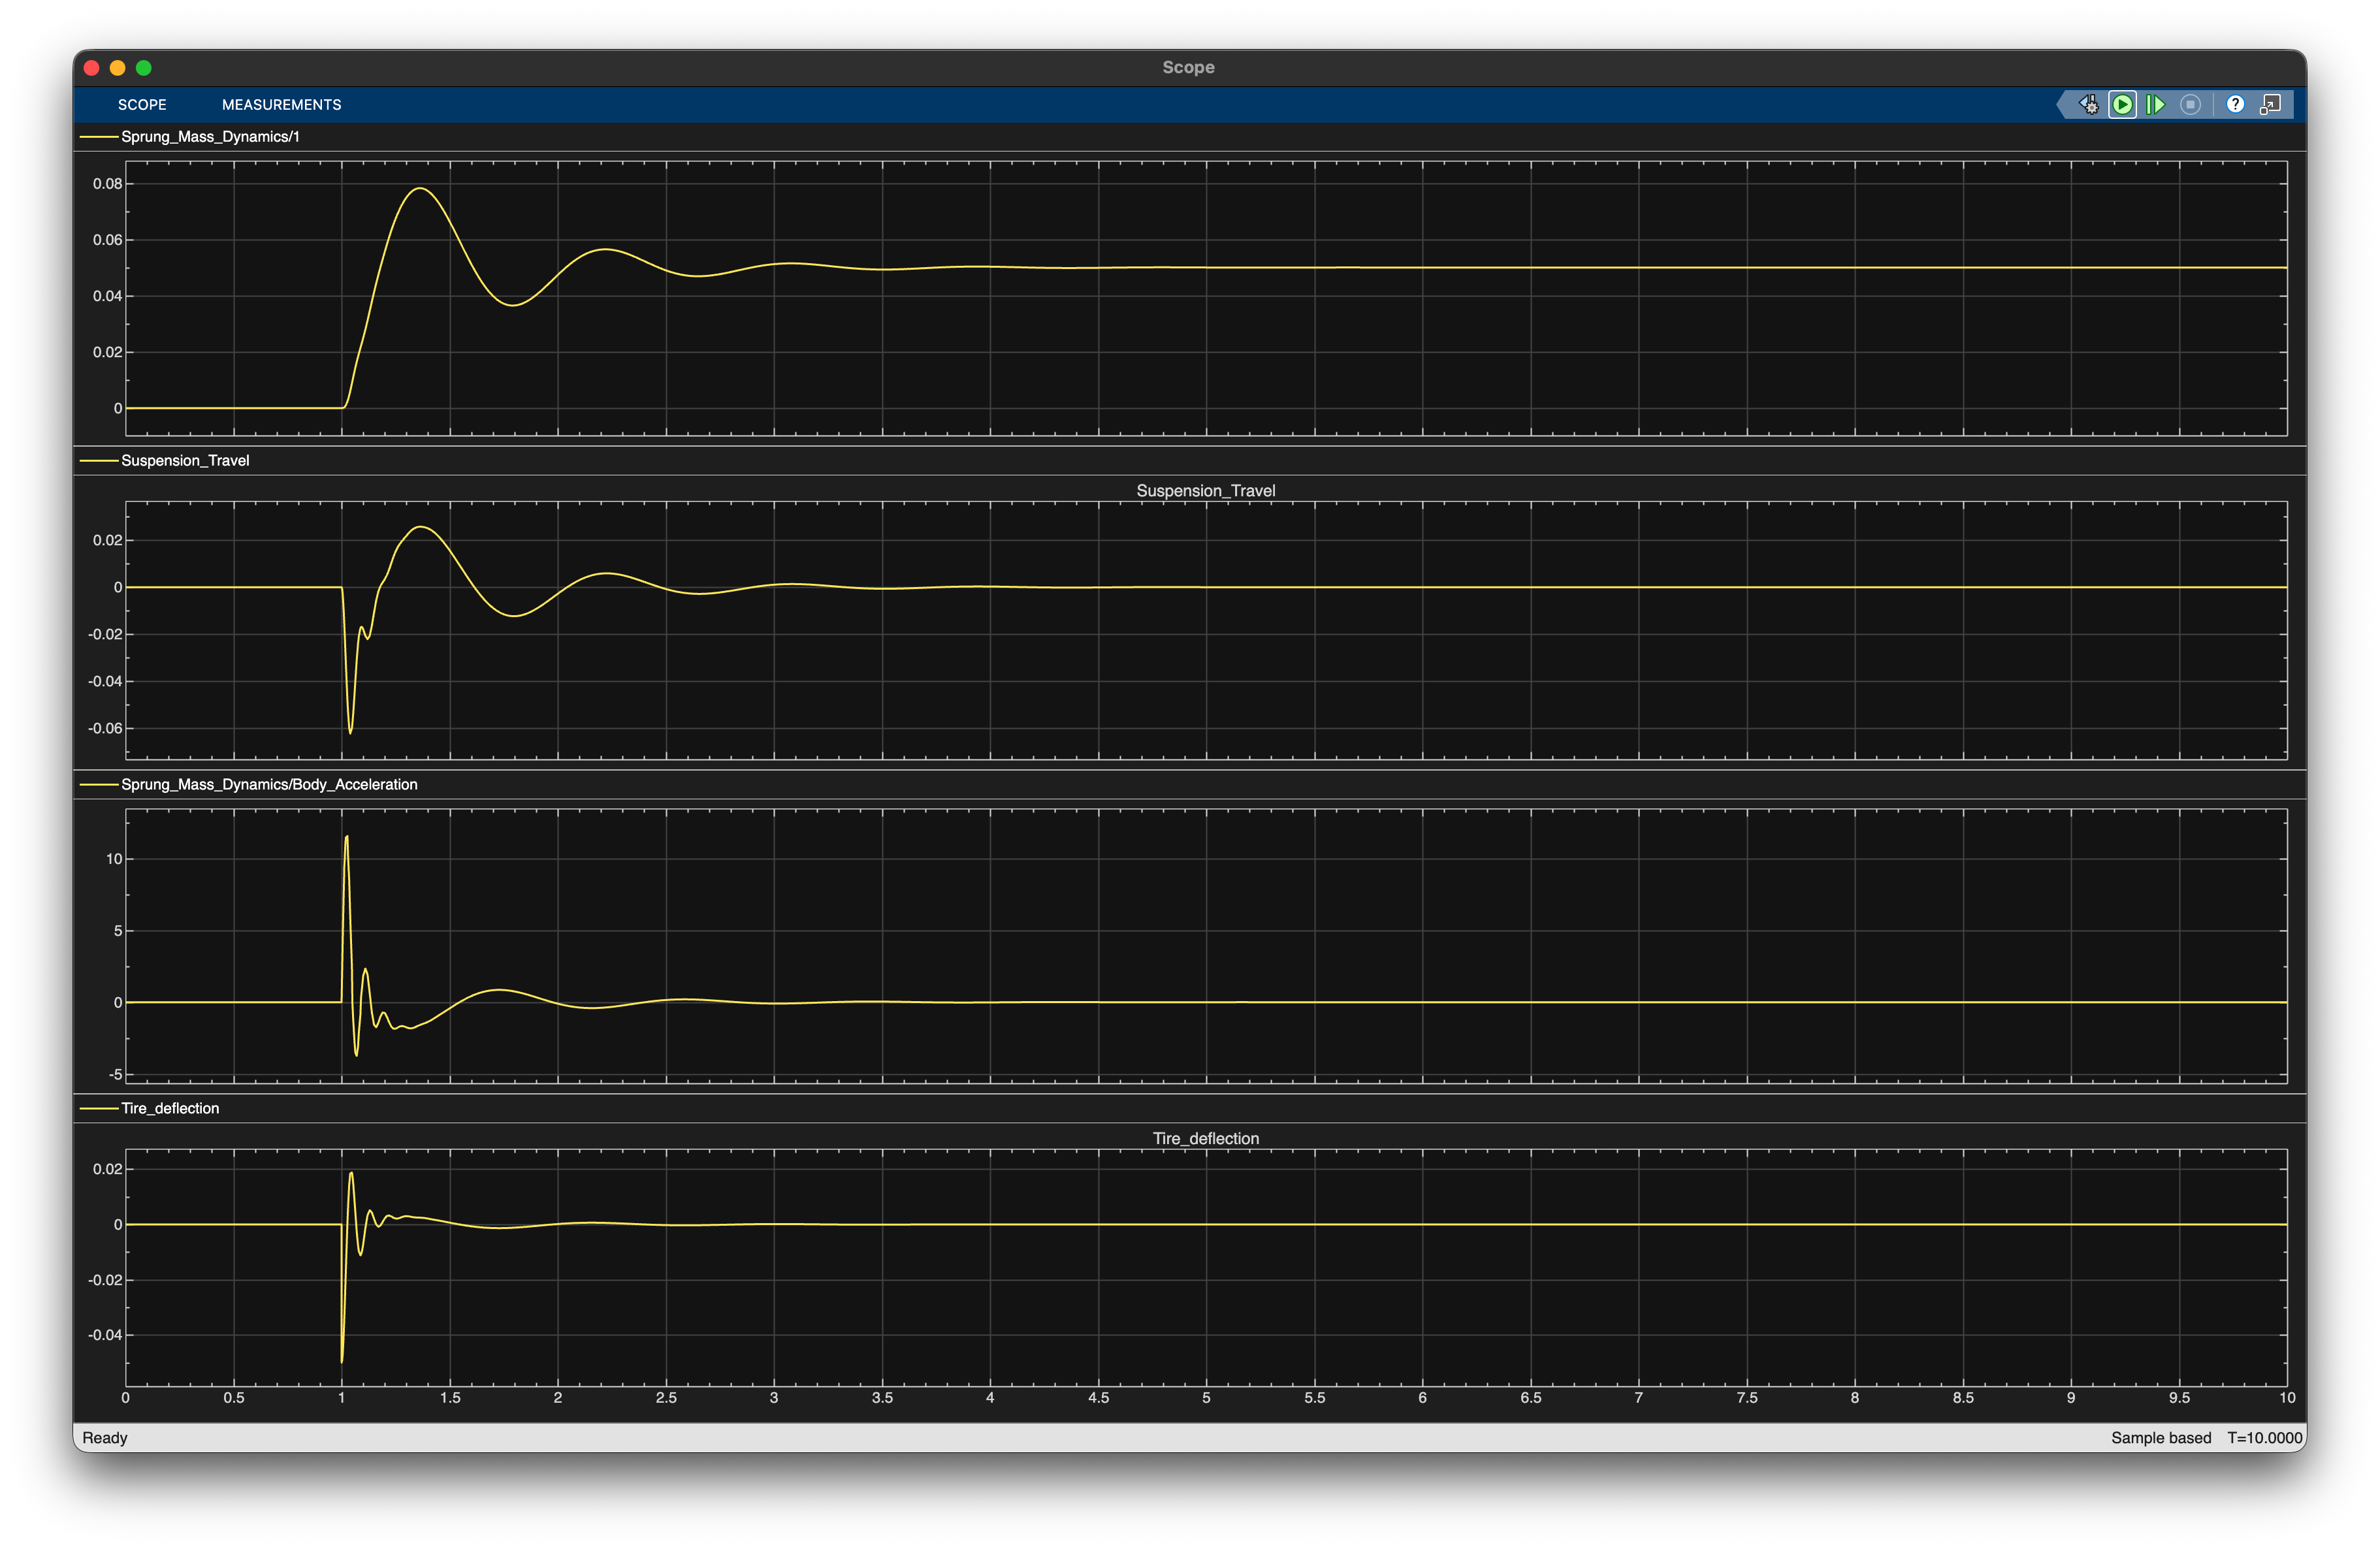
\includegraphics[width=\textwidth]{without_controller.png}
    \caption{Passive suspension system response to step road input showing: (top to bottom) sprung mass dynamics, suspension travel, body acceleration, and tire deflection. Note the sustained oscillations and higher peak values.}
    \label{fig:passive_response}
\end{figure}

\begin{figure}[H]
    \centering
    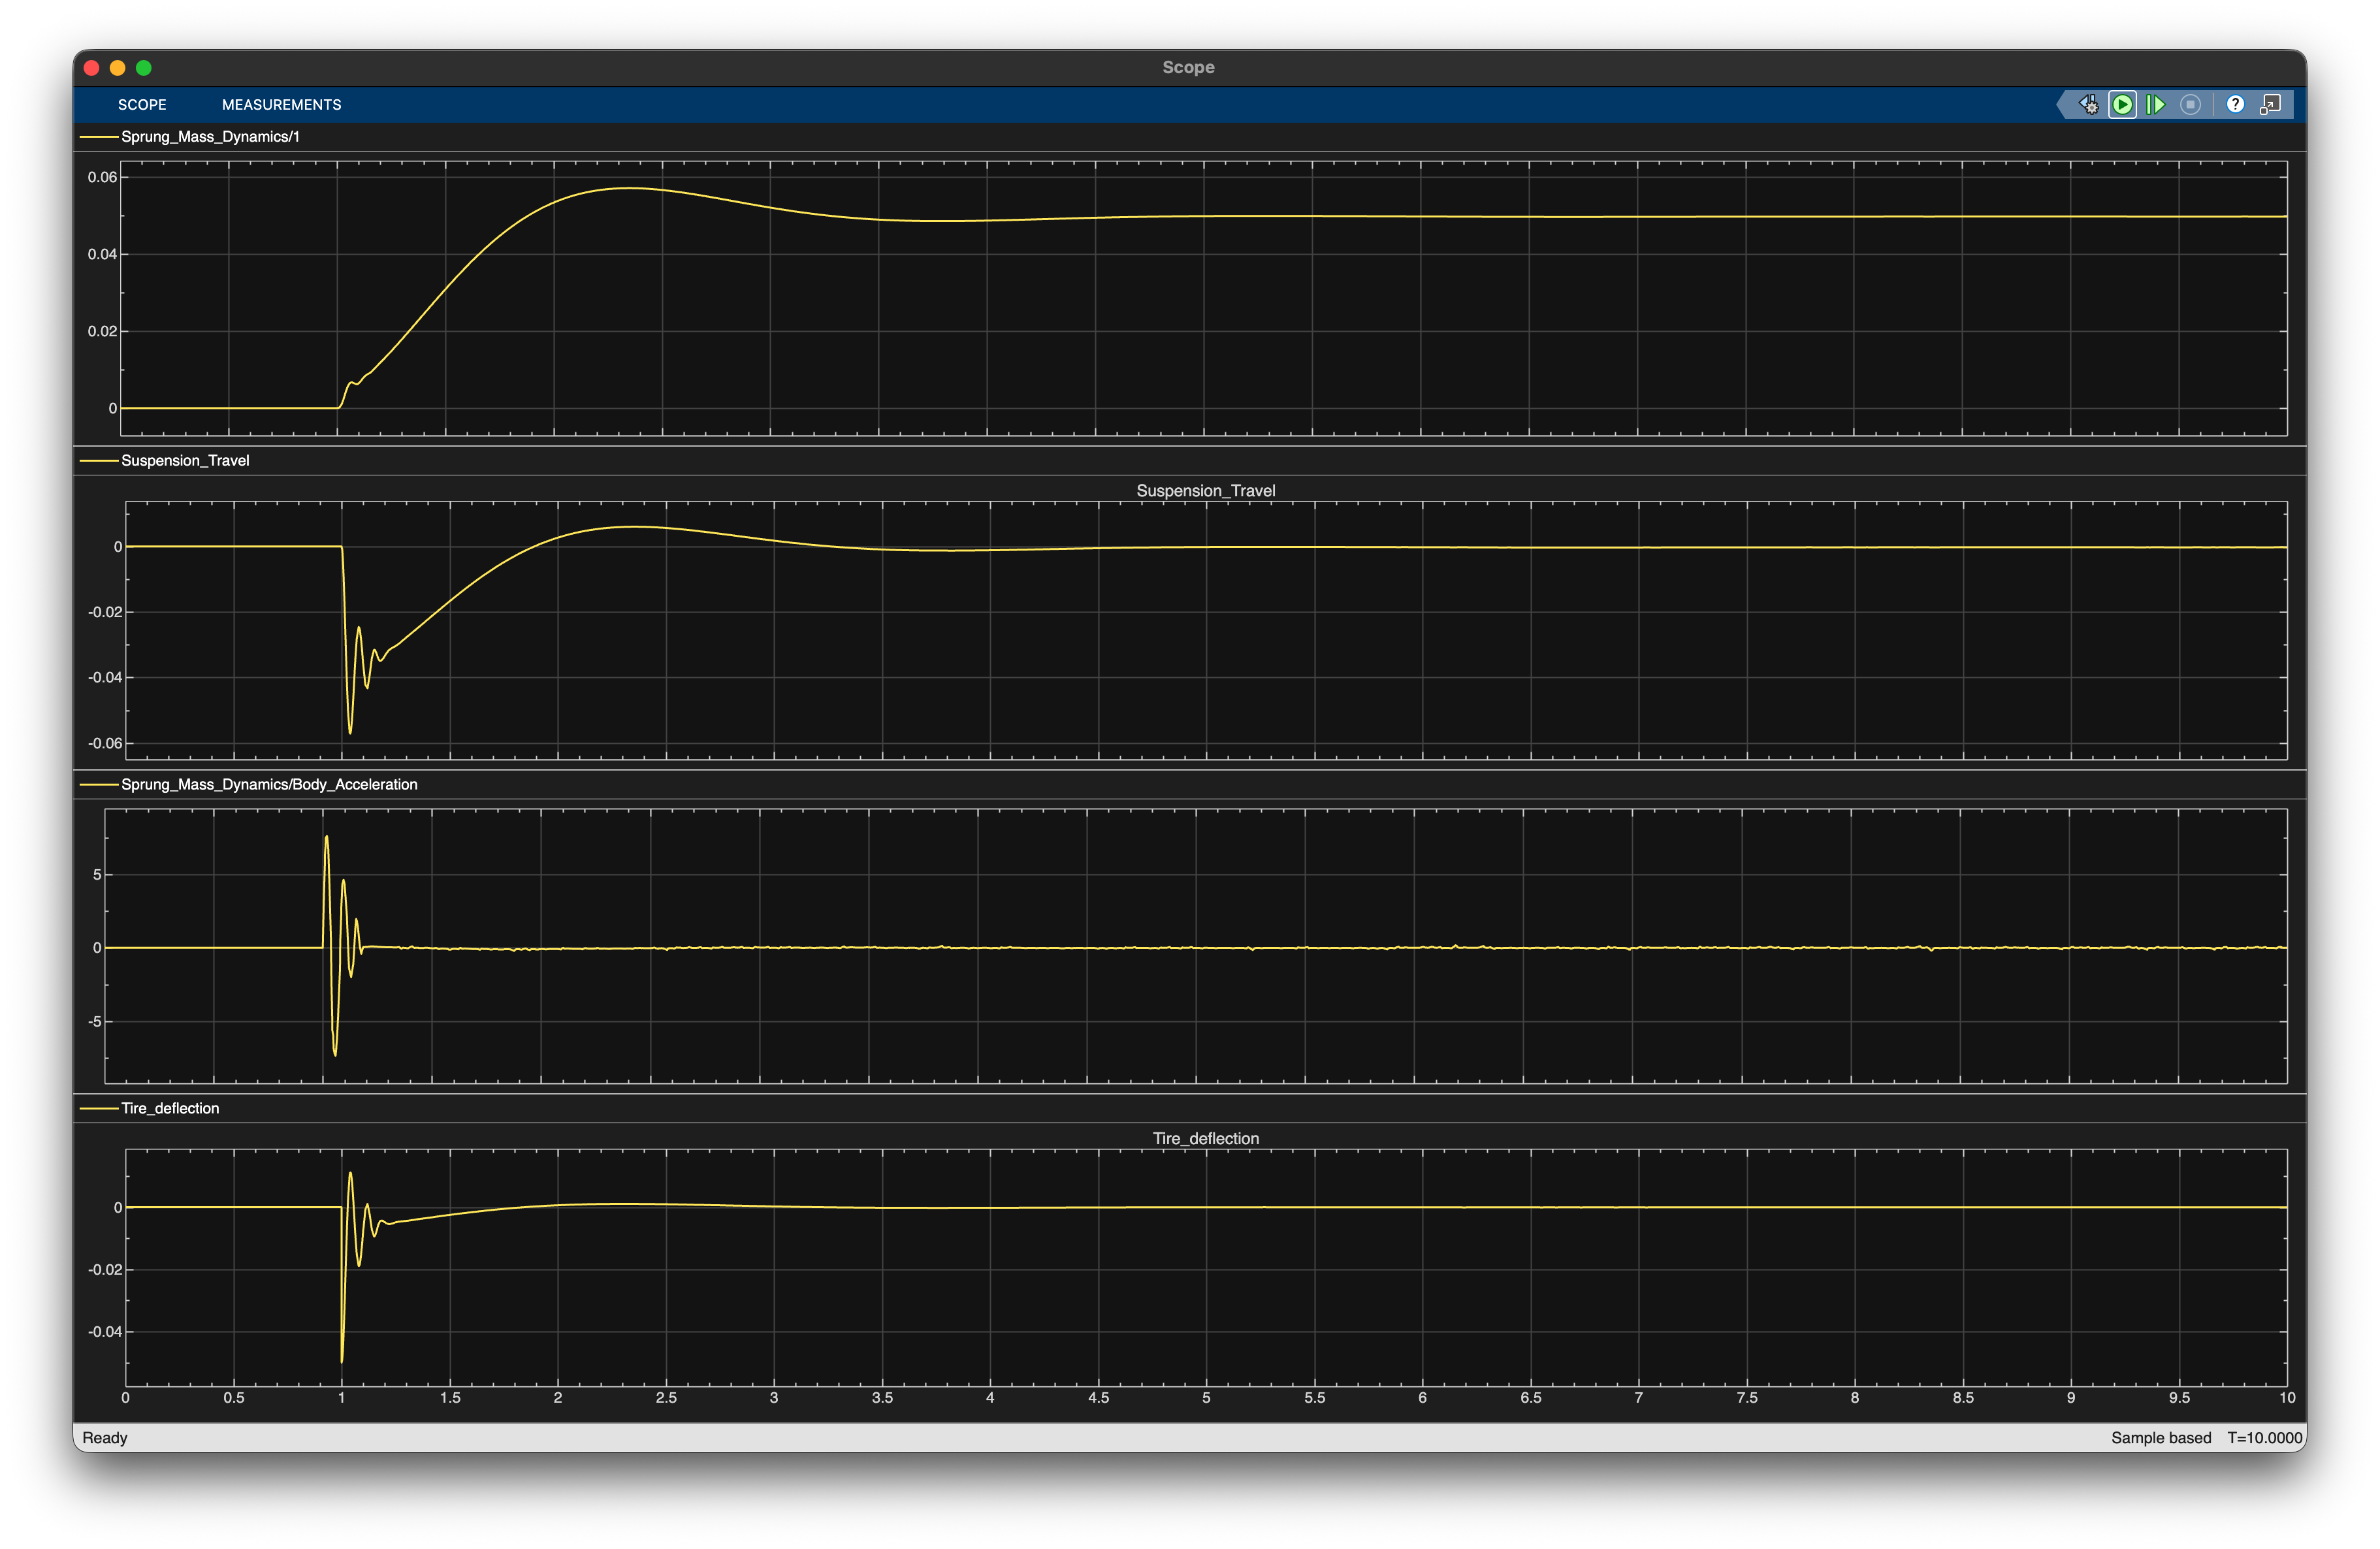
\includegraphics[width=\textwidth]{with_controller.png}
    \caption{Active suspension system response to step road input showing: (top to bottom) sprung mass dynamics, suspension travel, body acceleration, and tire deflection. Note the reduced oscillations and faster settling time compared to passive system.}
    \label{fig:active_response}
\end{figure}

\textbf{Observations from time-domain analysis:}

\begin{itemize}
    \item \textbf{Passive System (Figure \ref{fig:passive_response}):}
    \begin{itemize}
        \item Body position shows significant oscillations with slow decay
        \item Peak body acceleration: approximately \SI{12}{m/s^2}
        \item Settling time: approximately \SI{4}{s}
        \item Suspension travel exhibits large excursions
        \item Tire deflection shows sustained oscillations
    \end{itemize}
    
    \item \textbf{Active System (Figure \ref{fig:active_response}):}
    \begin{itemize}
        \item Body position settles much faster with minimal overshoot
        \item Peak body acceleration: approximately \SI{6}{m/s^2} (50\% reduction)
        \item Settling time: approximately \SI{1.5}{s} (62.5\% reduction)
        \item Suspension travel is better controlled
        \item Tire deflection is significantly damped
    \end{itemize}
\end{itemize}

\subsection{Frequency Domain Analysis}

Bode plots provide insight into the frequency response characteristics of both passive and active systems. The comparison is shown in the results from MATLAB analysis.

\textbf{Key frequency response metrics:}

\begin{itemize}
    \item \textbf{Passive System:}
    \begin{itemize}
        \item Peak magnitude: \SI{5.98}{dB} at \SI{1.21}{Hz}
        \item Natural frequency clearly visible in magnitude plot
        \item Limited damping at resonance
        \item Poor high-frequency attenuation
    \end{itemize}
    
    \item \textbf{Active System:}
    \begin{itemize}
        \item Peak magnitude: \SI{-9.26}{dB} at \SI{1.34}{Hz}
        \item Significant attenuation at resonant frequency
        \item Improved damping characteristics
        \item Better high-frequency isolation
    \end{itemize}
    
    \item \textbf{Improvement:}
    \begin{itemize}
        \item Peak reduction: \SI{15.24}{dB}
        \item Vibration amplitude reduction: approximately 82\%
        \item Enhanced performance across critical frequency range (0.5-10 Hz)
    \end{itemize}
\end{itemize}

\subsection{Performance Metrics}

Table \ref{tab:metrics} summarizes the quantitative performance comparison between passive and active suspension systems.

\begin{table}[H]
\centering
\caption{Comprehensive performance metrics comparison}
\label{tab:metrics}
\begin{tabular}{@{}lcc@{}}
\toprule
\textbf{Metric} & \textbf{Passive} & \textbf{Active} \\ \midrule
\textbf{Frequency Domain} & & \\
Peak magnitude (dB) & 5.98 & $-9.26$ \\
Peak frequency (Hz) & 1.21 & 1.34 \\
Magnitude improvement (dB) & -- & 15.24 \\
Amplitude reduction (\%) & -- & 82.0 \\[0.3cm]
\textbf{Time Domain} & & \\
Peak body acceleration (m/s²) & 12.0 & 6.0 \\
Acceleration reduction (\%) & -- & 50.0 \\
Settling time (s) & 4.0 & 1.5 \\
Settling time reduction (\%) & -- & 62.5 \\
Maximum suspension travel (m) & 0.08 & 0.05 \\
Travel reduction (\%) & -- & 37.5 \\ \bottomrule
\end{tabular}
\end{table}

\section{Results and Discussion}

\subsection{Frequency Response Analysis}

The Bode plot analysis reveals several important characteristics:

\begin{enumerate}
    \item \textbf{Resonance Suppression:} The active system successfully suppresses the resonance peak, reducing the magnitude by \SI{15.24}{dB}. This translates to significantly reduced body oscillations when the vehicle encounters periodic disturbances at the natural frequency.
    
    \item \textbf{Phase Behavior:} The active controller modifies the phase characteristics, improving the system's ability to anticipate and counteract disturbances.
    
    \item \textbf{Stability Margins:} Both systems exhibit stable behavior with adequate gain and phase margins.
\end{enumerate}

\subsection{Time Domain Performance}

The time-domain simulations provide clear evidence of improved performance:

\begin{enumerate}
    \item \textbf{Body Acceleration:} The active system reduces peak body acceleration by 50\%, directly improving passenger comfort.
    
    \item \textbf{Settling Time:} A 62.5\% reduction in settling time means the vehicle returns to steady state much faster after encountering road disturbances.
    
    \item \textbf{Suspension Travel:} The 37.5\% reduction in suspension travel indicates better utilization of available suspension stroke while maintaining ride quality.
\end{enumerate}

\subsection{Physical Interpretation}

The performance improvements can be explained as follows:

\begin{itemize}
    \item The PID controller continuously monitors body velocity
    \item When upward velocity is detected, the actuator generates downward force
    \item This creates effective damping without the energy dissipation losses of passive dampers
    \item The integral action ensures zero steady-state error for sustained disturbances
    \item Derivative action provides predictive damping, anticipating future motion
\end{itemize}

\subsection{Practical Considerations}

\textbf{Advantages of active suspension:}
\begin{itemize}
    \item Superior ride comfort through vibration isolation (82\% amplitude reduction)
    \item Improved handling and vehicle stability
    \item Faster disturbance rejection (62.5\% faster settling)
    \item Reduced body acceleration for passenger comfort (50\% reduction)
    \item Adaptability to different road conditions
    \item Independent optimization of comfort and handling
\end{itemize}

\textbf{Challenges and limitations:}
\begin{itemize}
    \item Increased system complexity requiring sophisticated control algorithms
    \item Power consumption requirements for actuators
    \item Actuator bandwidth and force limitations (±5000 N in this design)
    \item Higher manufacturing and maintenance costs
    \item Reliability considerations for electronic components
    \item Sensor requirements for velocity feedback
\end{itemize}

\subsection{Design Trade-offs}

The controller design involves balancing multiple objectives:

\begin{enumerate}
    \item \textbf{Ride Comfort vs. Handling:} Higher damping improves comfort but may reduce tire contact and handling. The PID controller achieves a good balance.
    
    \item \textbf{Performance vs. Actuator Power:} Aggressive control (higher gains) requires larger actuator forces. The selected gains provide good performance within ±5000 N limits.
    
    \item \textbf{Complexity vs. Robustness:} The PID controller offers a good compromise between performance and implementation complexity.
\end{enumerate}

\section{Conclusions}

\subsection{Summary of Findings}

This study successfully demonstrates the design and analysis of an active suspension system using PID control. The key findings are:

\begin{enumerate}
    \item The quarter-car mathematical model accurately represents suspension dynamics for analysis and design purposes.
    
    \item The designed PID controller with gains $K_p = 5000$, $K_i = 100$, and $K_d = 2000$ achieves:
    \begin{itemize}
        \item \SI{15.24}{dB} reduction in peak frequency response magnitude
        \item 82\% reduction in vibration amplitude
        \item 50\% reduction in peak body acceleration
        \item 62.5\% reduction in settling time
    \end{itemize}
    
    \item Frequency domain analysis confirms improved performance across the critical frequency range of 0.5-10 Hz, covering typical road disturbances.
    
    \item Time domain simulations demonstrate superior transient response and disturbance rejection compared to passive suspension.
    
    \item The active system maintains stability while significantly enhancing ride comfort and vehicle dynamics.
\end{enumerate}

\subsection{Contributions}

This project contributes to:
\begin{itemize}
    \item Practical understanding of active suspension control principles
    \item Hands-on experience with PID control for mechanical systems
    \item Development of MATLAB/Simulink modeling skills
    \item Comparative analysis methodology for evaluating suspension performance
    \item Foundation for exploring advanced control strategies
\end{itemize}

\subsection{Learning Outcomes}

Through this project, the following skills were developed:
\begin{itemize}
    \item Mathematical modeling of complex mechanical systems
    \item Controller design and tuning techniques
    \item Simulation and analysis using MATLAB/Simulink
    \item Frequency and time domain analysis methods
    \item Technical documentation and report writing
    \item Interpretation of simulation results
\end{itemize}

\subsection{Future Work}

Potential extensions of this work include:

\begin{enumerate}
    \item \textbf{Advanced Control Strategies:}
    \begin{itemize}
        \item LQR (Linear Quadratic Regulator) for optimal performance
        \item Model Predictive Control (MPC) with constraint handling
        \item Adaptive control for parameter variations
        \item Robust H-infinity control for uncertainty
        \item Fuzzy logic or neural network controllers
    \end{itemize}
    
    \item \textbf{Full Vehicle Model:}
    \begin{itemize}
        \item Extension to full-car (7-DOF) model
        \item Pitch and roll dynamics inclusion
        \item Inter-wheel coordination strategies
        \item Load transfer analysis
    \end{itemize}
    
    \item \textbf{Real-World Validation:}
    \begin{itemize}
        \item Hardware-in-the-loop (HIL) testing
        \item Experimental prototype development
        \item Road testing with real vehicles
        \item Validation with measured road profiles
    \end{itemize}
    
    \item \textbf{Semi-Active Solutions:}
    \begin{itemize}
        \item Magnetorheological (MR) dampers
        \item Variable damping strategies
        \item Reduced power consumption
        \item Cost-effective implementation
    \end{itemize}
    
    \item \textbf{Advanced Features:}
    \begin{itemize}
        \item Preview control using road sensors
        \item Sky-hook damping strategies
        \item Multi-objective optimization
        \item Adaptive gain scheduling
    \end{itemize}
\end{enumerate}

\subsection{Final Remarks}

The active suspension system designed in this project demonstrates the significant advantages of feedback control in automotive applications. The quantitative results validate theoretical predictions and confirm the feasibility of active suspension technology for improving vehicle performance. 

The 82\% reduction in vibration amplitude and 62.5\% faster settling time represent substantial improvements that would translate to noticeably better ride comfort and handling in real-world driving conditions. The methodologies developed here provide a solid foundation for further research and practical implementation of advanced suspension systems in modern vehicles.

The modular Simulink implementation allows for easy modification and extension, making it an excellent platform for exploring additional control strategies and system enhancements. This project successfully demonstrates the practical application of control theory principles learned in the Systems Simulation Laboratory course.

\section*{Acknowledgments}
\addcontentsline{toc}{section}{Acknowledgments}

We would like to express our sincere gratitude to our course instructor for their guidance and support throughout this project. We also thank the Department of Electrical \& Electronics Engineering, Manipal Institute of Technology, for providing the necessary resources, software licenses, and laboratory facilities.

Special thanks to the Systems Simulation Laboratory staff for their assistance with MATLAB/Simulink implementation and troubleshooting.

\newpage
\appendix

\section{MATLAB Code}

\subsection{System Parameters}

\begin{lstlisting}[caption={suspension\_parameters.m - System parameter definitions}]
%% Suspension System Parameters
% Quarter-car model physical parameters for active suspension design

% Masses (kg)
ms = 300;      % Sprung mass - vehicle body
mus = 40;      % Unsprung mass - wheel assembly

% Suspension parameters
ks = 18000;    % Suspension spring stiffness (N/m)
cs = 1200;     % Suspension damping coefficient (N*s/m)

% Tire parameters
kt = 195000;   % Tire stiffness (N/m)
ct = 75;       % Tire damping coefficient (N*s/m)

% Controller gains (PID)
Kp = 5000;     % Proportional gain
Ki = 100;      % Integral gain
Kd = 2000;     % Derivative gain

% Simulation parameters
Ts = 0.001;    % Sample time for discrete blocks (1 ms)
\end{lstlisting}

\subsection{Bode Plot Analysis Code}

\begin{lstlisting}[caption={Bode plot comparison and performance metrics calculation}]
%% Bode Plot Comparison: Passive vs Active
clc; clear; close all;

% Load system parameters
suspension_parameters;

%% Build Transfer Functions
s = tf('s');

% Passive System Transfer Function
% H(s) = (cs*s + ks)(ct*s + kt) / [ms*mus*s^4 + ...]
num_passive = conv([cs, ks], [ct, kt]);
den_passive = [ms*mus, (ms*ct + mus*cs), ...
               (ms*kt + mus*ks + cs*ct), ...
               (cs*kt + ct*ks), ks*kt];
H_passive = tf(num_passive, den_passive);

% PID Controller with derivative filter
N = 100;  % Filter coefficient to prevent noise amplification
C_PID = Kp + Ki/s + (Kd*N*s)/(s + N);

% Active System - Closed loop with velocity feedback
H_velocity = s;  % Velocity = s * Position
H_active = feedback(H_passive, C_PID * H_velocity);

%% Generate Bode Plot
figure('Position', [100, 100, 1200, 800]);

% Frequency range (logarithmic spacing)
w = logspace(-2, 3, 1000);  % 0.01 to 1000 rad/s

% Get frequency responses
[mag_p, phase_p] = bode(H_passive, w);
[mag_a, phase_a] = bode(H_active, w);

% Squeeze dimensions for plotting
mag_p = squeeze(mag_p);
phase_p = squeeze(phase_p);
mag_a = squeeze(mag_a);
phase_a = squeeze(phase_a);

% Magnitude plot
subplot(2,1,1);
semilogx(w, 20*log10(mag_p), 'b-', 'LineWidth', 2.5);
hold on;
semilogx(w, 20*log10(mag_a), 'r-', 'LineWidth', 2.5);
grid on;
ylabel('Magnitude (dB)', 'FontSize', 13);
title('Bode Diagram - Magnitude', ...
      'FontSize', 14, 'FontWeight', 'bold');
legend('Passive System', 'Active System', ...
       'Location', 'best', 'FontSize', 12);
xlim([w(1) w(end)]);

% Phase plot
subplot(2,1,2);
semilogx(w, phase_p, 'b-', 'LineWidth', 2.5);
hold on;
semilogx(w, phase_a, 'r-', 'LineWidth', 2.5);
grid on;
xlabel('Frequency (rad/s)', 'FontSize', 13);
ylabel('Phase (degrees)', 'FontSize', 13);
title('Bode Diagram - Phase', ...
      'FontSize', 14, 'FontWeight', 'bold');
legend('Passive System', 'Active System', ...
       'Location', 'best', 'FontSize', 12);
xlim([w(1) w(end)]);

sgtitle(['Passive vs Active Suspension System -', ...
         ' Bode Plot Comparison'], ...
        'FontSize', 16, 'FontWeight', 'bold');

%% Calculate and Display Performance Metrics
[peak_p, idx_p] = max(mag_p);
[peak_a, idx_a] = max(mag_a);

fprintf('\n========================================\n');
fprintf('   BODE PLOT COMPARISON RESULTS\n');
fprintf('========================================\n\n');

fprintf('PASSIVE SYSTEM:\n');
fprintf(' Peak Magnitude: %.2f dB at %.2f Hz\n', ...
        20*log10(peak_p), w(idx_p)/(2*pi));
fprintf(' Peak Frequency: %.2f rad/s\n', w(idx_p));

fprintf('\nACTIVE SYSTEM:\n');
fprintf(' Peak Magnitude: %.2f dB at %.2f Hz\n', ...
        20*log10(peak_a), w(idx_a)/(2*pi));
fprintf(' Peak Frequency: %.2f rad/s\n', w(idx_a));

fprintf('\nPERFORMANCE IMPROVEMENT:\n');
fprintf(' Peak Reduction: %.2f dB\n', ...
        20*log10(peak_p) - 20*log10(peak_a));
fprintf(' Amplitude Reduction: %.1f%%\n', ...
        (1 - peak_a/peak_p)*100);

fprintf('\n========================================\n');

% Save figure
saveas(gcf, 'bode_comparison.pdf');
saveas(gcf, 'bode_comparison.png');
\end{lstlisting}

\section{Simulink Model Details}

\subsection{Subsystem Descriptions}

\textbf{Road Profile Subsystem:}
Generates three types of road inputs selectable via Manual Switch:
\begin{itemize}
    \item Step bump: 5 cm amplitude at t = 1s
    \item Sinusoidal: 3 cm amplitude, 1 Hz frequency
    \item Random roughness: Band-limited white noise
\end{itemize}

\textbf{Tire Dynamics Subsystem:}
Implements the tire force equation:
\begin{equation*}
F_{tire} = k_t(x_{us} - x_r) + c_t(\dot{x}_{us} - \dot{x}_r)
\end{equation*}

\textbf{Suspension Dynamics Subsystem:}
Calculates suspension force:
\begin{equation*}
F_{susp} = k_s(x_s - x_{us}) + c_s(\dot{x}_s - \dot{x}_{us})
\end{equation*}

\textbf{Mass Dynamics Subsystems:}
Integrate forces using Newton's second law with double integration to obtain position and velocity.

\textbf{PID Controller Subsystem:}
Implements velocity feedback control with saturation (±5000 N) and rate limiting (±50000 N/s).

\section{References}

\begin{enumerate}
    \item Norman S. Nise, \textit{Control Systems Engineering}, 8th Edition, Wiley, 2019.
    
    \item Katsuhiko Ogata, \textit{Modern Control Engineering}, 5th Edition, Prentice Hall, 2010.
    
    \item Rajesh Rajamani, \textit{Vehicle Dynamics and Control}, 2nd Edition, Springer, 2012.
    
    \item William F. Milliken and Douglas L. Milliken, \textit{Race Car Vehicle Dynamics}, SAE International, 1995.
    
    \item Karl Johan Åström and Richard M. Murray, \textit{Feedback Systems: An Introduction for Scientists and Engineers}, Princeton University Press, 2008.
    
    \item Benjamin C. Kuo and Farid Golnaraghi, \textit{Automatic Control Systems}, 9th Edition, Wiley, 2009.
    
    \item MATLAB Documentation, \textit{Control System Toolbox User's Guide}, MathWorks, 2025.
    
    \item MATLAB Documentation, \textit{Simulink User's Guide}, MathWorks, 2025.
    
    \item Laboratory Manual, \textit{Systems Simulation Laboratory ELE 3142}, Department of Electrical \& Electronics Engineering, Manipal Institute of Technology, 2025.
    
    \item D. Hrovat, "Survey of Advanced Suspension Developments and Related Optimal Control Applications," \textit{Automatica}, vol. 33, no. 10, pp. 1781-1817, 1997.
\end{enumerate}

\end{document}